% Backup of remote conflict block from origin/main during merge on results.tex
% Keeping this file to ensure no content is lost.

% Remote block 1 (duplicate of combined contamination rates figure)
\begin{figure}[htbp]
    \centering
    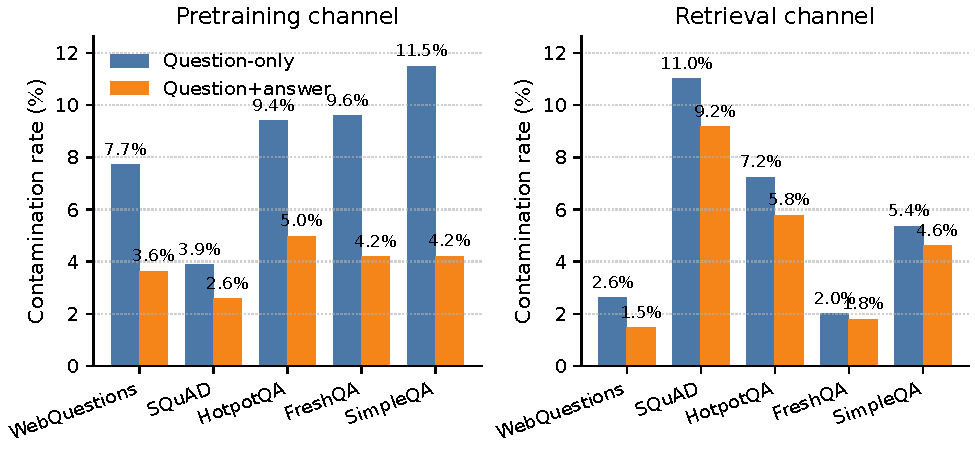
\includegraphics[width=\columnwidth]{res/contamination_rates_by_dataset_combined.pdf}
    \caption{Contamination rates by dataset across the two leakage channels defined in the modeling framework: (a) pretraining contamination (source set $\mathcal{S}_{\text{pre}}{=}D_M$), and (b) retrieval-time contamination (source set $\mathcal{S}_{\text{ret}}{=}\mathcal{R}(q)$).}
    \label{fig:contamination_rates_by_dataset_remote}
\end{figure}

% Remote block 2 (side-by-side minipage layout)
\begin{figure}[htbp]
    \centering
    \begin{minipage}[t]{0.49\columnwidth}
        \centering
        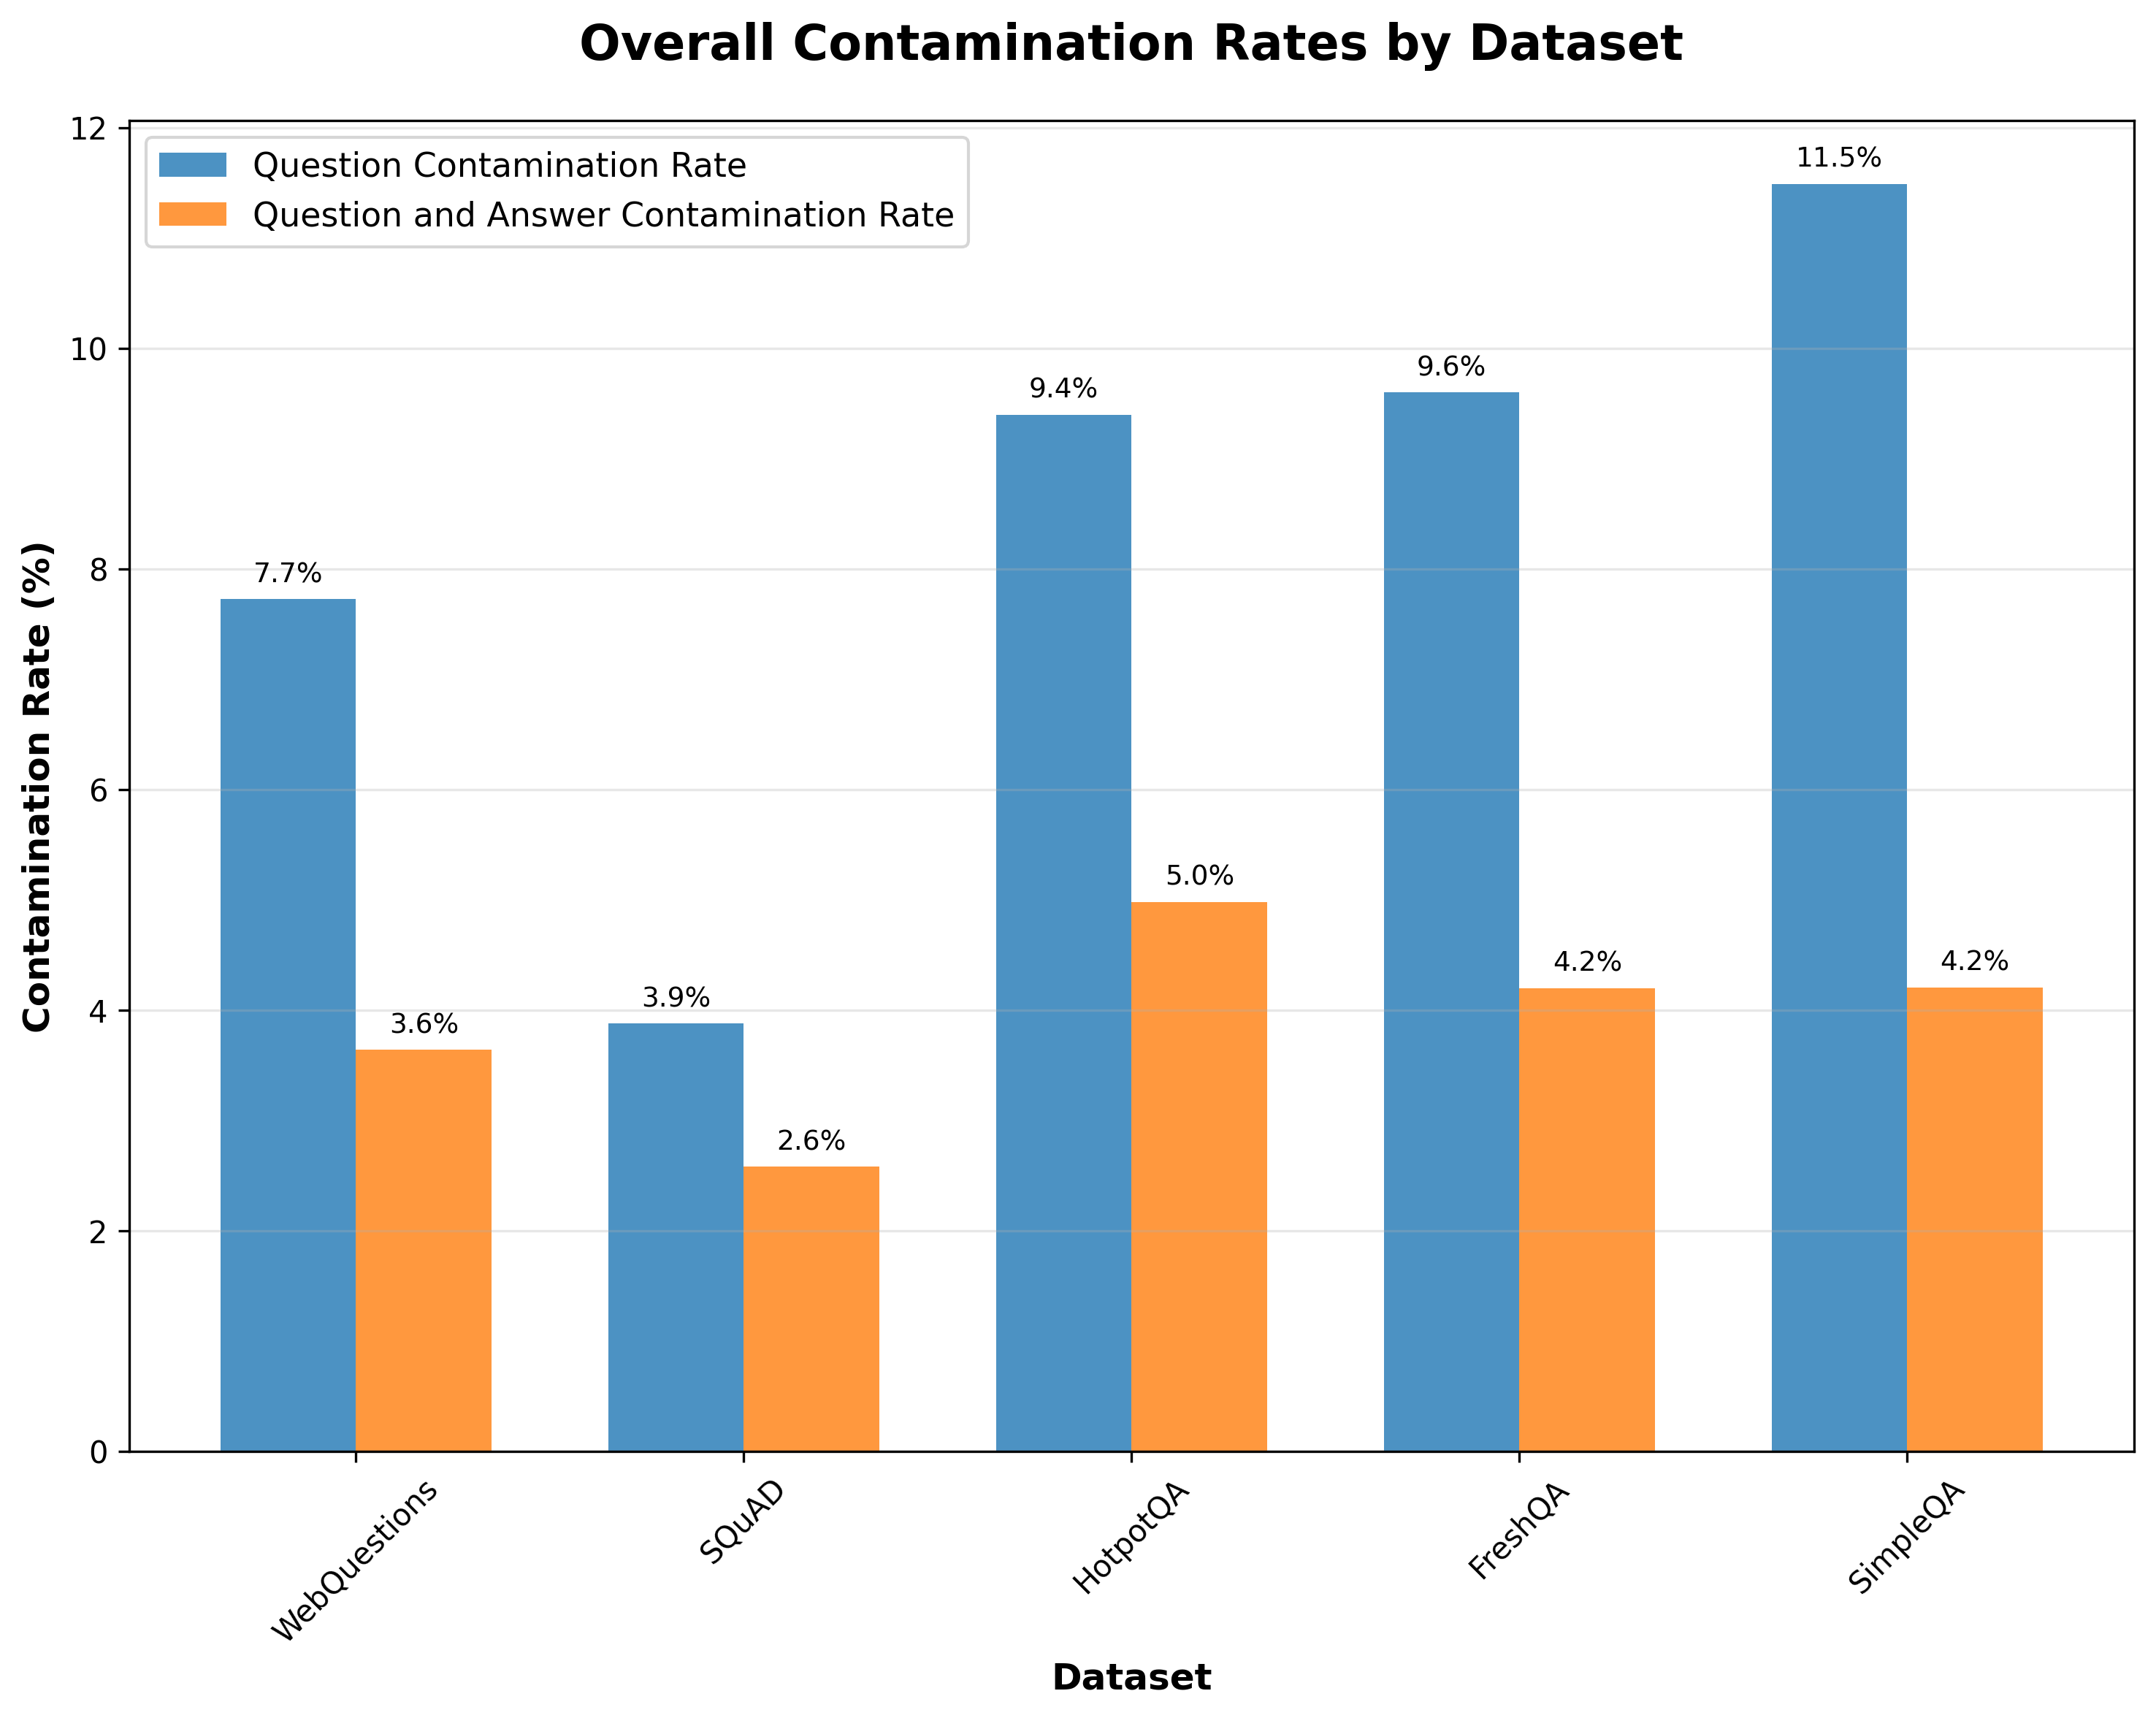
\includegraphics[width=\columnwidth]{from_sandeep/plots_and_interpretations_contamination/analysis_20250831_221700/overall_contamination_rates_by_dataset.png}
        \\[4pt]
        {\small (a) Pretraining channel: contamination rates by dataset}
    \end{minipage}\hfill
    \begin{minipage}[t]{0.49\columnwidth}
        \centering
        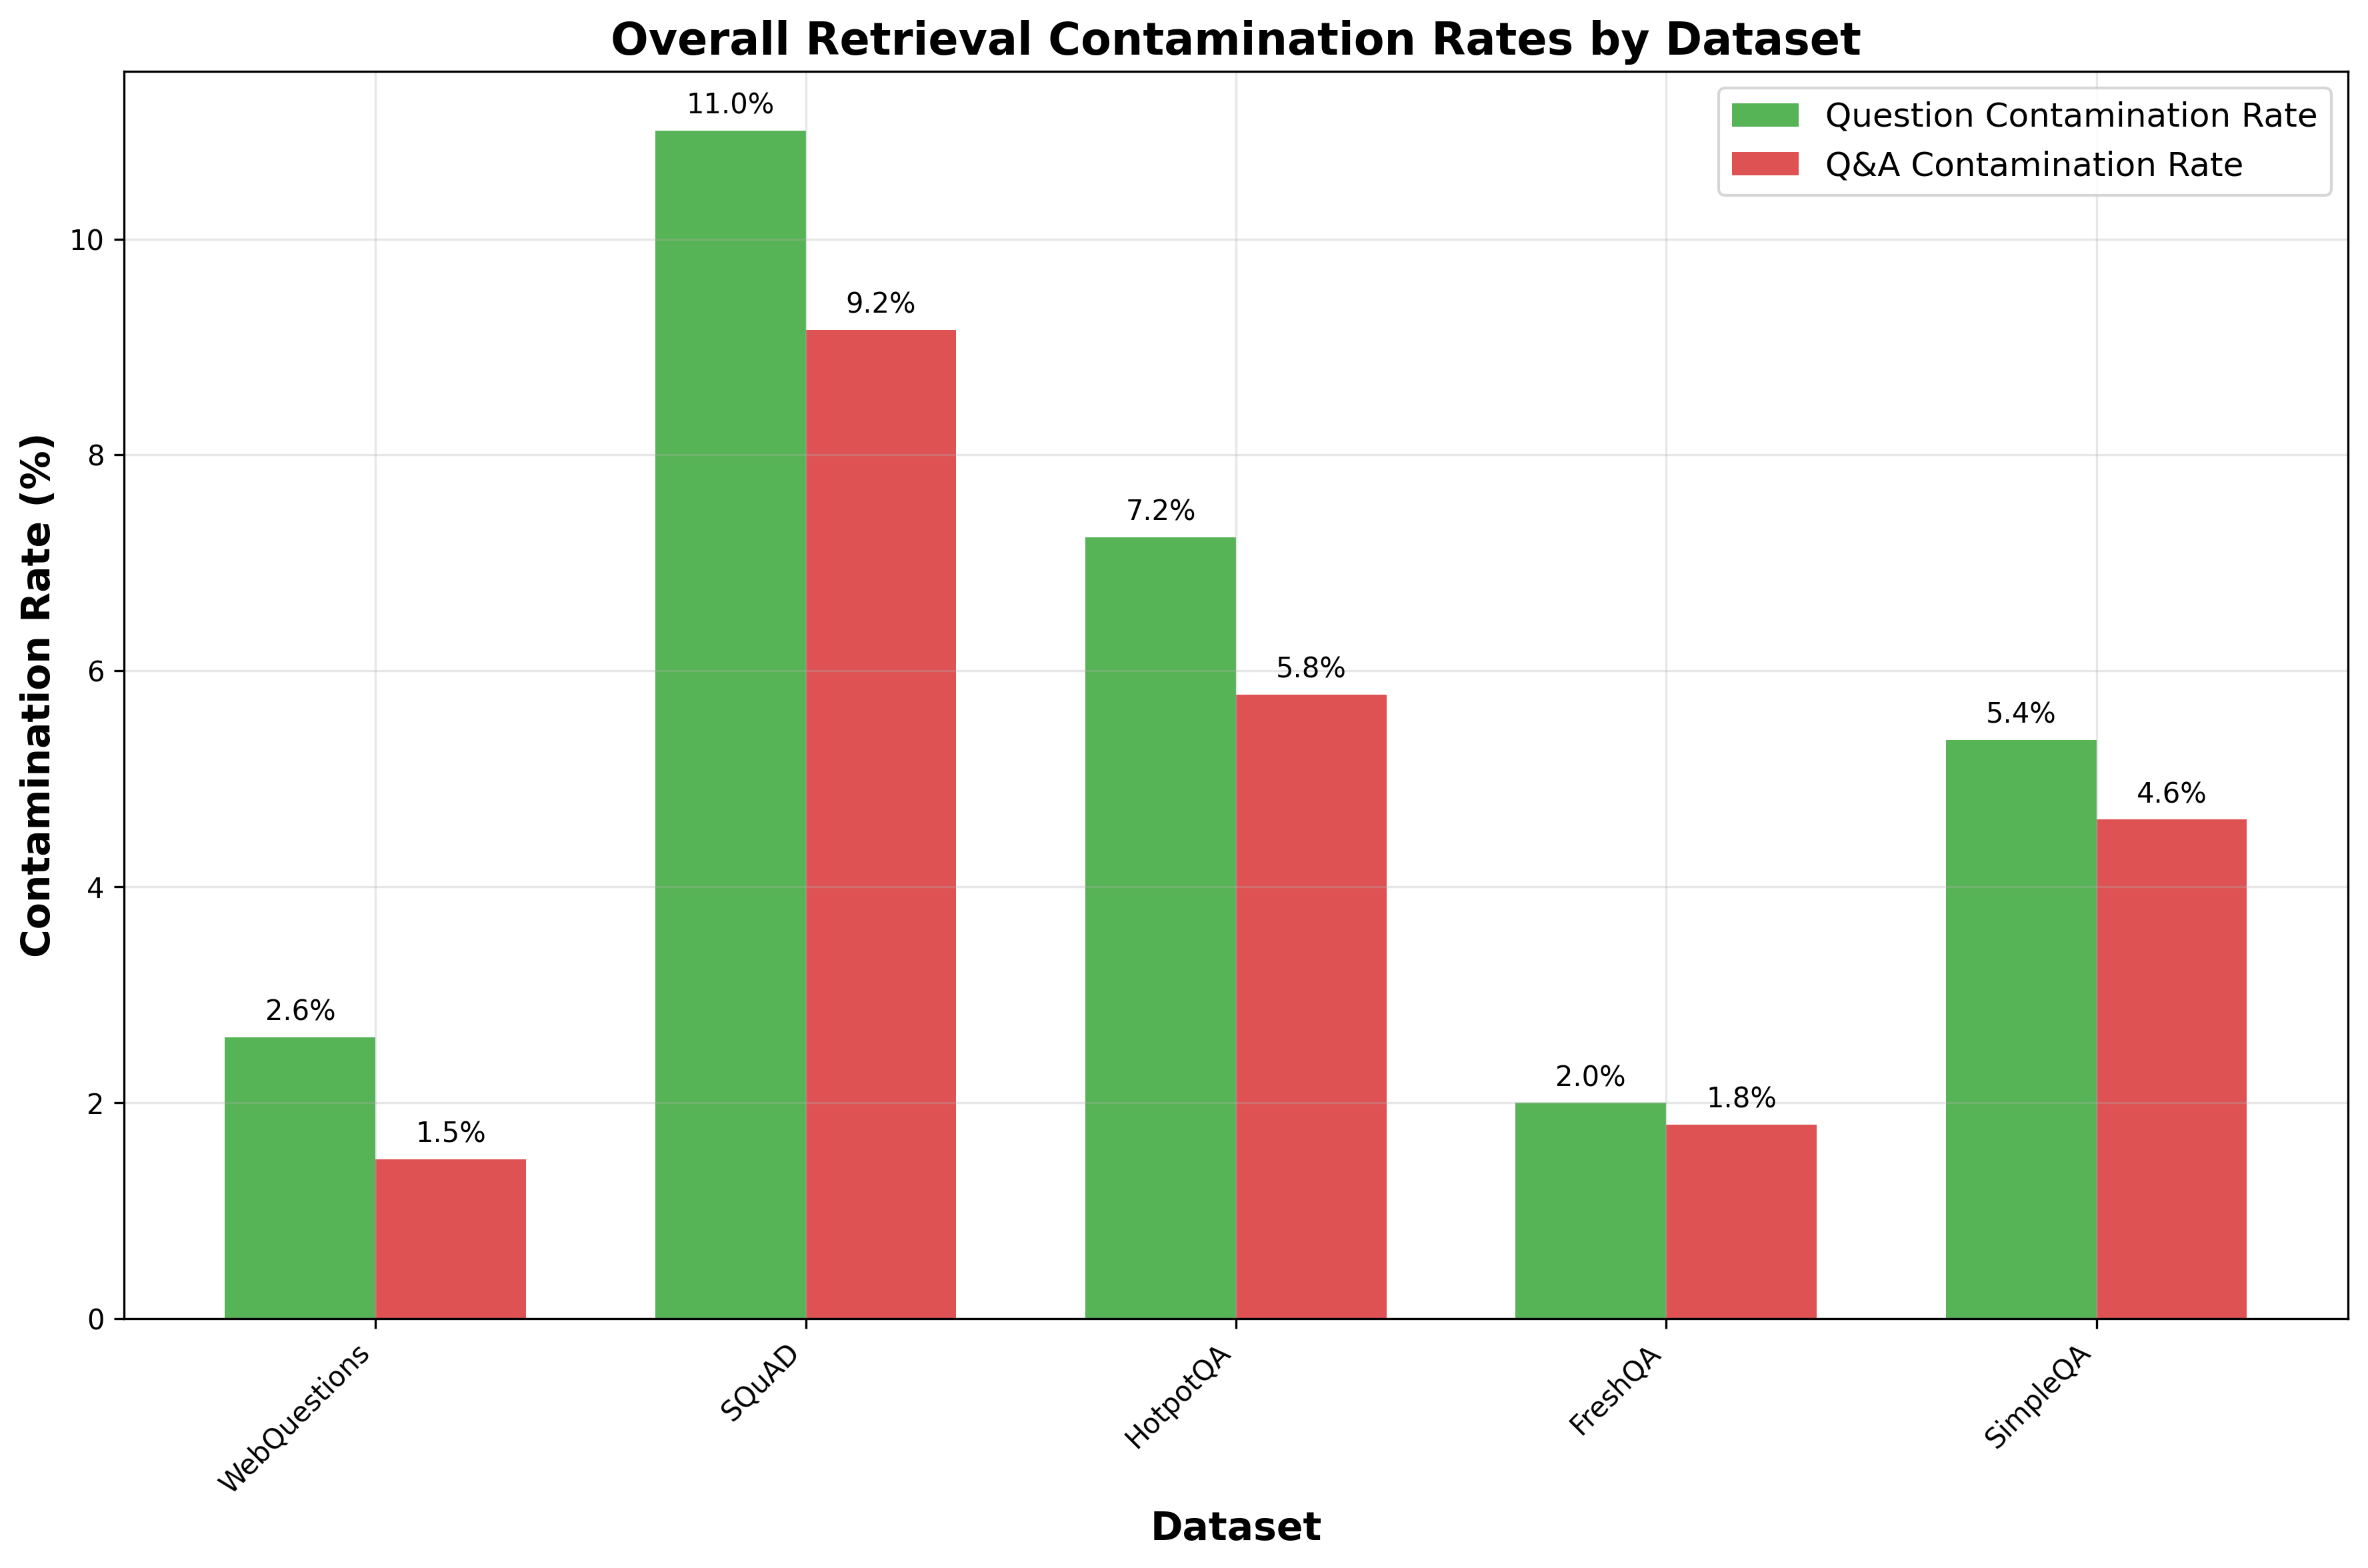
\includegraphics[width=\columnwidth]{from_sandeep/plots_and_interpretations_contamination/overall_retrieval_analysis_20250831_221712/overall_retrieval_contamination_rates_by_dataset.png}
        \\[4pt]
        {\small (b) Retrieval-time channel (web-RAG): contamination rates by dataset}
    \end{minipage}
    \caption{Side-by-side contamination rates across leakage channels (backup from remote).}
    \label{fig:contamination_rates_by_dataset_side_by_side_backup}
\end{figure}


